% !TeX spellcheck = en_US
\addsection{AI Rules}{\spells/fortune.png}

\iftoggle{printable}{\vspace{-\baselineskip}}{}

\begin{multicols}{2}

\subsection*{AI Hero Turn}
\pagetarget{AIrules}{AI Heroes} are used in the Campaigns.
They start in their Town, and have 3 MP, always spending them to perform the following Actions in descending priority:
\begin{itemize}
  \item If a player's Hero is on the same Tile as the AI, spend all MP to move towards them in an attempt to start Combat.
  \item If there are any Mines or Settlements the AI could Flag on the same Tile, move towards the closest one.
  \item Otherwise, move toward the player's Town.
Repeat this sequence until all MPs are used up.
AI Heroes take their turn after the player.
\end{itemize}

AI Heroes always \textbf{automatically win Combat} against any Neutral Units, while simultaneously \textbf{Flagging or Visiting all Fields} they happen to move through.
They gain no benefits from any Fields.

AI Heroes must discover face down Map Tiles as normal by spending 1 MP before moving onto them.
The player chooses that Tile's orientation.\par
AI Heroes cannot Surrender and you cannot Surrender to them;
they will always fight until they run out of Units.
Winning Combat against an AI Hero does not grant any rewards unless stated by the Scenario.
AI Heroes do not have a Town Board, Resources, or a Hero Card.
Their Units are static and defined by the Scenario's setup or other rules.\par
Any differences to the above will be described in any given Scenario's own rules.
\vfill

\subsection*{AI Decks}

\begin{multicols*}{2}
  \begin{center}
    \vspace*{-1.5em}
    \begin{tikzpicture}
      \draw (0, 0) node {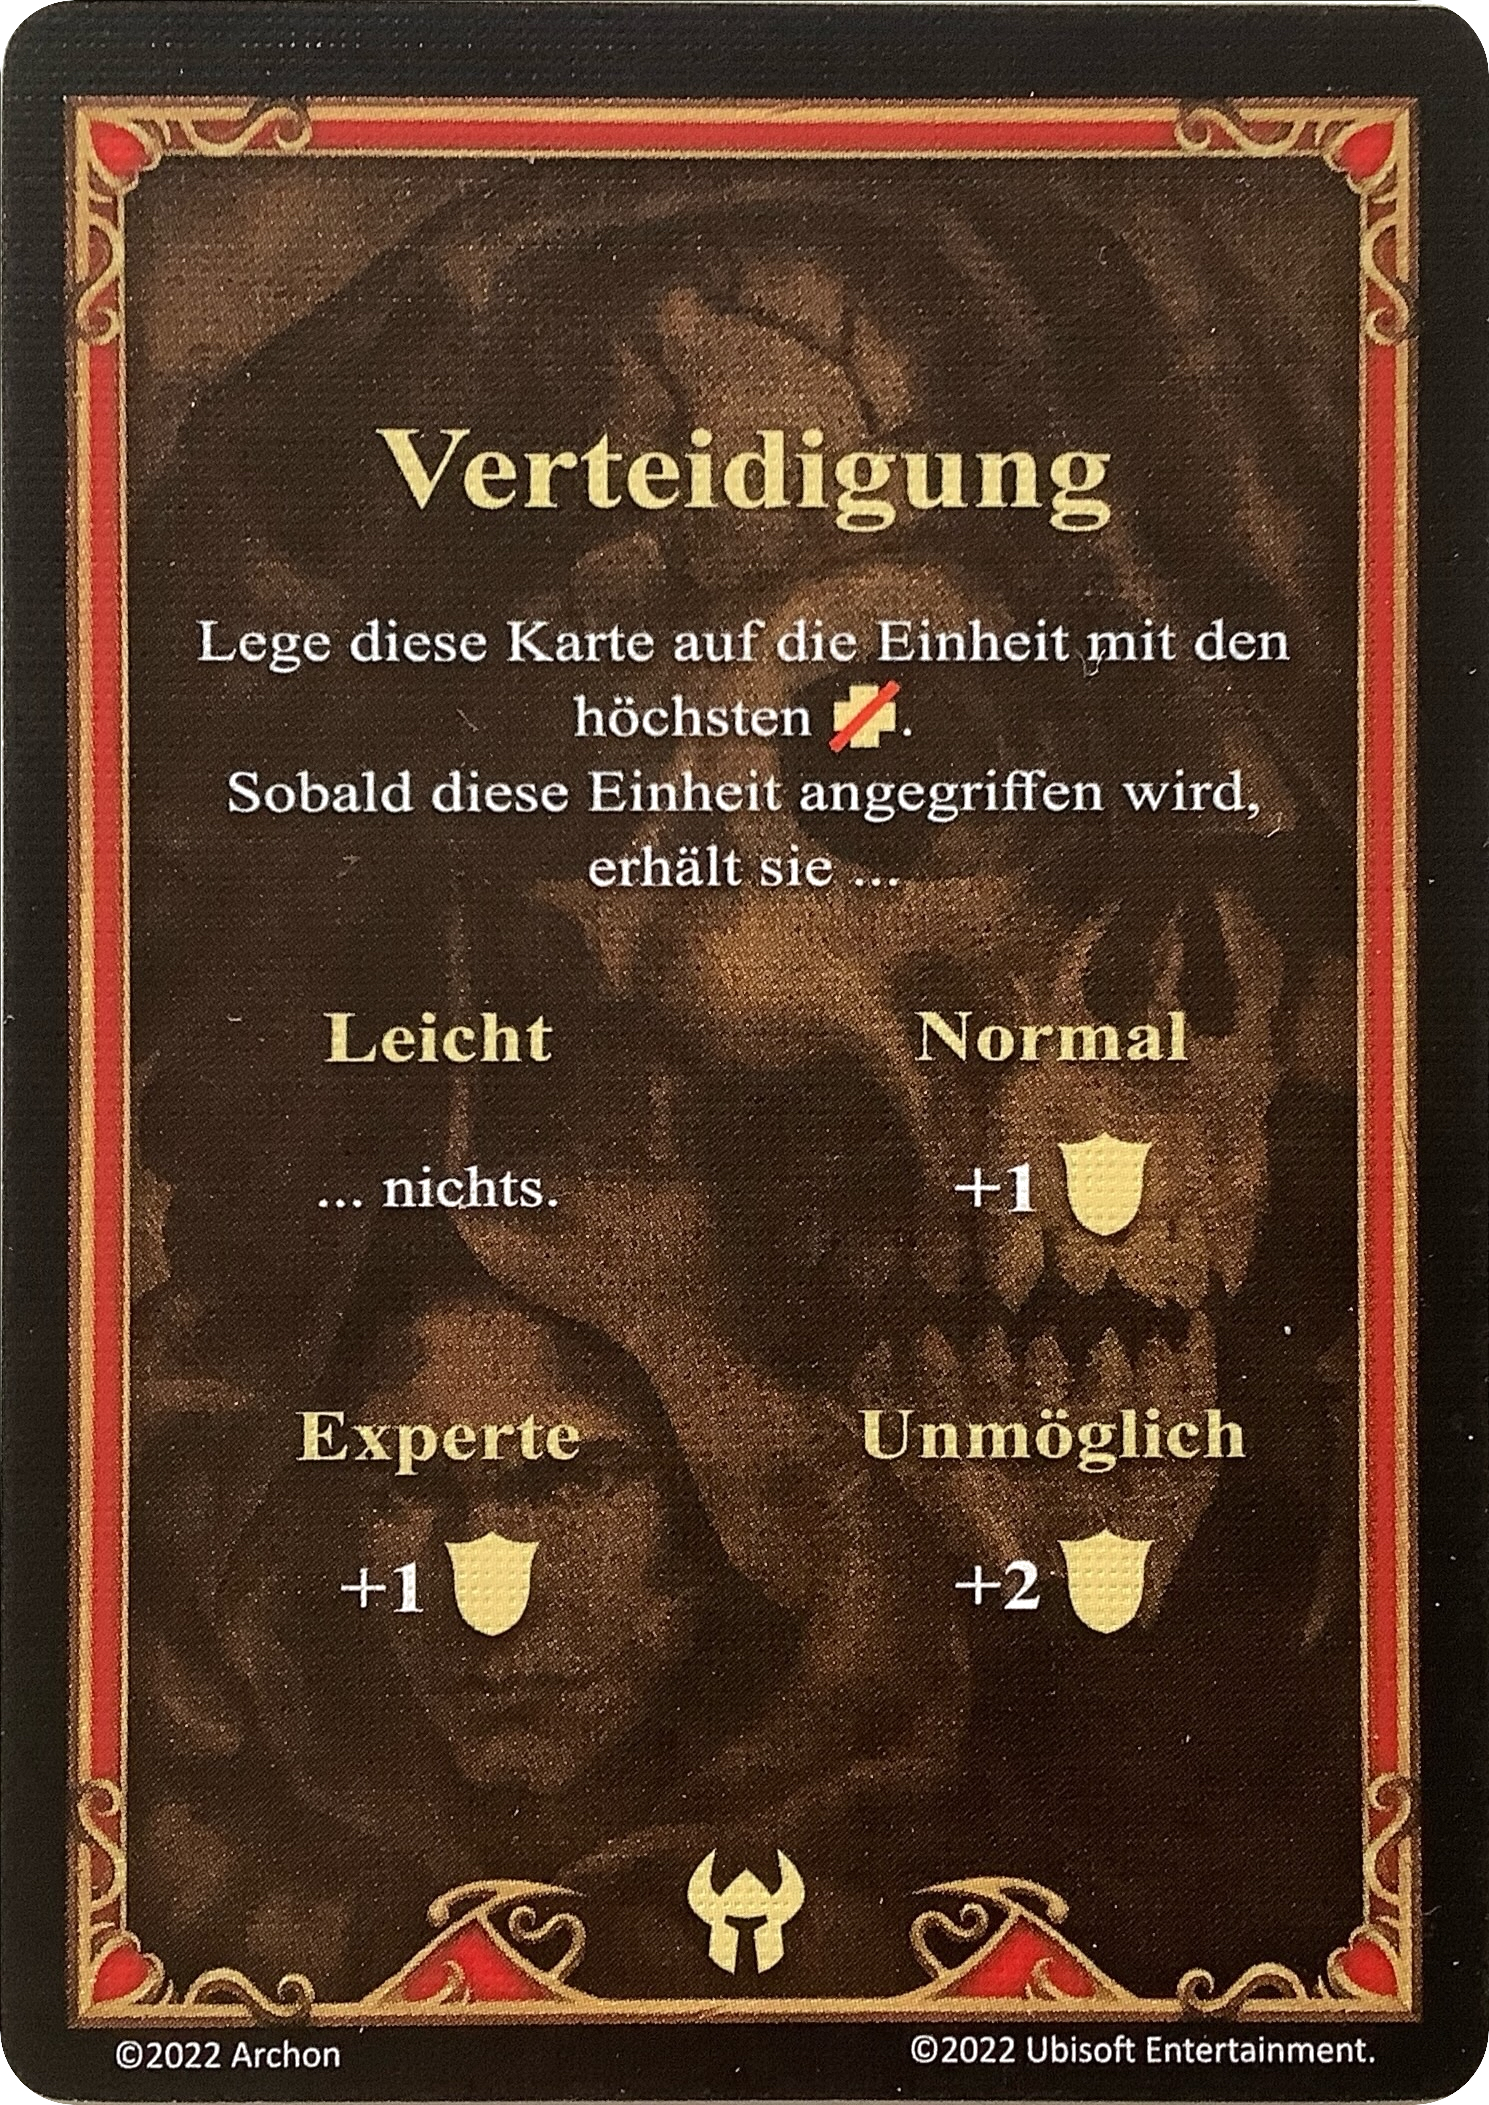
\includegraphics[width=1.3\linewidth]{\cards/ai.png}};
      \draw (-0.7, 2.5) node {\encircle{1}};
      \draw (1.5, 1.2) node {\encircle{2}};
      \draw (-1.5, 0) node {\encircle{3}};
      \draw (0.5, 0) node {\encircle{4}};
      \draw (-1.5, -1.2) node {\encircle{5}};
      \draw (0.5, -1.2) node {\encircle{6}};
      \draw (-0.5, -2.5) node {\encircle{7}};
    \end{tikzpicture}\\
    \phantom{\ldots\ldots}\footnotesize{\textbf{\textit{\textcolor{darkcandyapplered}{AI Card}}}}
    \vspace*{-1em}
  \end{center}
  \vspace*{\fill}
  \columnbreak
  \scriptsize
  \begin{itemize}[itemsep=0pt]
    \item[\textbf{1.}] Name
    \item[\textbf{2.}] Description
    \item[\textbf{3.}] Easy Modifier
    \item[\textbf{4.}] Normal Modifier
    \item[\textbf{5.}] Expert Modifier
    \item[\textbf{6.}] Impossible\\Modifier
    \item[\textbf{7.}] Card Type
  \end{itemize}\vspace*{\fill}
\end{multicols*}

AI Heroes use two Decks during Combat: the \textbf{AI Deck}, and the \textbf{AI Spell Deck}.
The AI Deck consists of three types of AI cards: Might \svg{might}, Magic \svg{magic} and Skill \svg{skill}.
Each Campaign scenario lists the number and types of Cards to include during setup.
Choose these cards \textbf{randomly} when building the Deck.
If Skill Cards are included, search for and set aside the Ability Card related to it.
Build the \textbf{AI Spell Deck} by separating the indicated Spells from the regular Spell Deck.
Shuffle these Decks during setup after building them.

When an AI Hero \textbf{Activates} a Unit, draw an AI Card\index{AI Card} and follow its instructions before the Unit moves and/or attacks.
If AI Deck is depleted during Combat, stop drawing from it.
The effect of each AI card depends on the game's \pagelink{Difficulty}{Difficulty}.
The Might Card \svg{might} is attached to the unit until the first respective attack/defense happens.
The AI Spell Deck is used whenever a Magic Card \svg{magic} is drawn.
If an AI Hero is instructed to draw a card, they will draw and resolve \textbf{another card} from the AI Deck.

\subsection*{Combat against AI}

\pagetarget{AI Units}{These rules} apply during Combat in \textbf{Solo}\index{Solo Mode} and \textbf{Cooperative} Scenarios.
The rules for AI unit placement during setup are described in \pagelink{CombatAISetup}{Combat chapter}.

When Neutral enemies or AI Heroes activate a unit, they follow a set of automatic instructions:\par

\begin{itemize}
  \item Enemy Ground \svg{unit_ground} and Flying \svg{unit_flying} Units prioritize attacking Units of the \textbf{same} tier.
  If this is impossible, they attack the Unit of a lower tier (in tier \textbf{descending} order, down to bronze), and if that is also impossible, they attack the Unit of a higher tier (in tier \textbf{ascending} order).\par

  \textit{Example: \svgunit{golden}\svg{unit_ground} has this priority:
  \svgunit{golden}
  - \svgunit{silver}
  - \svgunit{bronze}
  - \svgunit{azure}.}

  \item Ranged \svg{unit_ranged} Units prioritize attacking other Ranged \svg{unit_ranged} Units of the same tier, then lower tier, and finally higher tier, using the same tier order as above.
  If there are no Ranged \svg{unit_ranged} Units for them to target, they prioritize Ground \svg{unit_ground} and Flying \svg{unit_flying} Units in the same tier order.\par

  \textit{Example: \svgunit{silver}\svg{unit_ranged} has this priority:
  \svgunit{silver}\svg{unit_ranged}
  - \svgunit{bronze}\svg{unit_ranged}
  - \svgunit{golden}\svg{unit_ranged}
  - \svgunit{azure}\svg{unit_ranged}
  - \svgunit{silver}\svg{unit_ground}\svg{unit_flying}
  - \svgunit{bronze}\svg{unit_ground}\svg{unit_flying}
  - \svgunit{golden}\svg{unit_ground}\svg{unit_flying}
  - \svgunit{azure}\svg{unit_ground}\svg{unit_flying}.}
\end{itemize}

In both cases, if there's more than one valid target, they attack the closest one.
If there's ever a tie between equally valid targets, the player chooses which Unit is attacked.\par

Enemy units cannot \pagelink{Defend}{Defend} unless instructed to.

\vfill

\begin{center}
    \includegraphics[width=\linewidth,height=\textheight,keepaspectratio]{\art/titan.jpg}
\end{center}

\end{multicols}
